\documentclass[twoside]{book}

% Packages required by doxygen
\usepackage{fixltx2e}
\usepackage{calc}
\usepackage{doxygen}
\usepackage[export]{adjustbox} % also loads graphicx
\usepackage{graphicx}
\usepackage[utf8]{inputenc}
\usepackage{makeidx}
\usepackage{multicol}
\usepackage{multirow}
\PassOptionsToPackage{warn}{textcomp}
\usepackage{textcomp}
\usepackage[nointegrals]{wasysym}
\usepackage[table]{xcolor}

% Font selection
\usepackage[T1]{fontenc}
\usepackage[scaled=.90]{helvet}
\usepackage{courier}
\usepackage{amssymb}
\usepackage{sectsty}
\renewcommand{\familydefault}{\sfdefault}
\allsectionsfont{%
  \fontseries{bc}\selectfont%
  \color{darkgray}%
}
\renewcommand{\DoxyLabelFont}{%
  \fontseries{bc}\selectfont%
  \color{darkgray}%
}
\newcommand{\+}{\discretionary{\mbox{\scriptsize$\hookleftarrow$}}{}{}}

% Page & text layout
\usepackage{geometry}
\geometry{%
  a4paper,%
  top=2.5cm,%
  bottom=2.5cm,%
  left=2.5cm,%
  right=2.5cm%
}
\tolerance=750
\hfuzz=15pt
\hbadness=750
\setlength{\emergencystretch}{15pt}
\setlength{\parindent}{0cm}
\setlength{\parskip}{3ex plus 2ex minus 2ex}
\makeatletter
\renewcommand{\paragraph}{%
  \@startsection{paragraph}{4}{0ex}{-1.0ex}{1.0ex}{%
    \normalfont\normalsize\bfseries\SS@parafont%
  }%
}
\renewcommand{\subparagraph}{%
  \@startsection{subparagraph}{5}{0ex}{-1.0ex}{1.0ex}{%
    \normalfont\normalsize\bfseries\SS@subparafont%
  }%
}
\makeatother

% Headers & footers
\usepackage{fancyhdr}
\pagestyle{fancyplain}
\fancyhead[LE]{\fancyplain{}{\bfseries\thepage}}
\fancyhead[CE]{\fancyplain{}{}}
\fancyhead[RE]{\fancyplain{}{\bfseries\leftmark}}
\fancyhead[LO]{\fancyplain{}{\bfseries\rightmark}}
\fancyhead[CO]{\fancyplain{}{}}
\fancyhead[RO]{\fancyplain{}{\bfseries\thepage}}
\fancyfoot[LE]{\fancyplain{}{}}
\fancyfoot[CE]{\fancyplain{}{}}
\fancyfoot[RE]{\fancyplain{}{\bfseries\scriptsize Generated by Doxygen }}
\fancyfoot[LO]{\fancyplain{}{\bfseries\scriptsize Generated by Doxygen }}
\fancyfoot[CO]{\fancyplain{}{}}
\fancyfoot[RO]{\fancyplain{}{}}
\renewcommand{\footrulewidth}{0.4pt}
\renewcommand{\chaptermark}[1]{%
  \markboth{#1}{}%
}
\renewcommand{\sectionmark}[1]{%
  \markright{\thesection\ #1}%
}

% Indices & bibliography
\usepackage{natbib}
\usepackage[titles]{tocloft}
\setcounter{tocdepth}{3}
\setcounter{secnumdepth}{5}
\makeindex

% Hyperlinks (required, but should be loaded last)
\usepackage{ifpdf}
\ifpdf
  \usepackage[pdftex,pagebackref=true]{hyperref}
\else
  \usepackage[ps2pdf,pagebackref=true]{hyperref}
\fi
\hypersetup{%
  colorlinks=true,%
  linkcolor=blue,%
  citecolor=blue,%
  unicode%
}

% Custom commands
\newcommand{\clearemptydoublepage}{%
  \newpage{\pagestyle{empty}\cleardoublepage}%
}

\usepackage{caption}
\captionsetup{labelsep=space,justification=centering,font={bf},singlelinecheck=off,skip=4pt,position=top}

%===== C O N T E N T S =====

\begin{document}

% Titlepage & ToC
\hypersetup{pageanchor=false,
             bookmarksnumbered=true,
             pdfencoding=unicode
            }
\pagenumbering{roman}
\begin{titlepage}
\vspace*{7cm}
\begin{center}%
{\Large RF Signal Map Android Application \\[1ex]\large 1.\+0 }\\
\vspace*{1cm}
{\large Generated by Doxygen 1.8.11}\\
\end{center}
\end{titlepage}
\clearemptydoublepage
\tableofcontents
\clearemptydoublepage
\pagenumbering{arabic}
\hypersetup{pageanchor=true}

%--- Begin generated contents ---
\chapter{Hierarchical Index}
\section{Class Hierarchy}
This inheritance list is sorted roughly, but not completely, alphabetically\+:\begin{DoxyCompactList}
\item \contentsline{section}{edu.\+tamu.\+rfsignalmap.\+Lat\+Long}{\pageref{classedu_1_1tamu_1_1rfsignalmap_1_1_lat_long}}{}
\item On\+Click\+Listener\begin{DoxyCompactList}
\item \contentsline{section}{edu.\+tamu.\+rfsignalmap.\+Main\+Activity\+Fragment}{\pageref{classedu_1_1tamu_1_1rfsignalmap_1_1_main_activity_fragment}}{}
\end{DoxyCompactList}
\item On\+Preference\+Change\+Listener\begin{DoxyCompactList}
\item \contentsline{section}{edu.\+tamu.\+rfsignalmap.\+Settings\+Fragment}{\pageref{classedu_1_1tamu_1_1rfsignalmap_1_1_settings_fragment}}{}
\end{DoxyCompactList}
\item \contentsline{section}{edu.\+tamu.\+rfsignalmap.\+R\+F\+Data}{\pageref{classedu_1_1tamu_1_1rfsignalmap_1_1_r_f_data}}{}
\item \contentsline{section}{edu.\+tamu.\+rfsignalmap.\+R\+F\+Field\+S\+Q\+L\+Database}{\pageref{classedu_1_1tamu_1_1rfsignalmap_1_1_r_f_field_s_q_l_database}}{}
\item App\+Compat\+Activity\begin{DoxyCompactList}
\item \contentsline{section}{edu.\+tamu.\+rfsignalmap.\+Main\+Activity}{\pageref{classedu_1_1tamu_1_1rfsignalmap_1_1_main_activity}}{}
\end{DoxyCompactList}
\item Fragment\begin{DoxyCompactList}
\item \contentsline{section}{edu.\+tamu.\+rfsignalmap.\+About\+Fragment}{\pageref{classedu_1_1tamu_1_1rfsignalmap_1_1_about_fragment}}{}
\item \contentsline{section}{edu.\+tamu.\+rfsignalmap.\+Main\+Activity\+Fragment}{\pageref{classedu_1_1tamu_1_1rfsignalmap_1_1_main_activity_fragment}}{}
\item \contentsline{section}{edu.\+tamu.\+rfsignalmap.\+Maps\+View\+Fragment}{\pageref{classedu_1_1tamu_1_1rfsignalmap_1_1_maps_view_fragment}}{}
\end{DoxyCompactList}
\item Location\+Listener\begin{DoxyCompactList}
\item \contentsline{section}{edu.\+tamu.\+rfsignalmap.\+Main\+Activity\+Fragment}{\pageref{classedu_1_1tamu_1_1rfsignalmap_1_1_main_activity_fragment}}{}
\end{DoxyCompactList}
\item On\+Map\+Click\+Listener\begin{DoxyCompactList}
\item \contentsline{section}{edu.\+tamu.\+rfsignalmap.\+Maps\+View\+Fragment}{\pageref{classedu_1_1tamu_1_1rfsignalmap_1_1_maps_view_fragment}}{}
\end{DoxyCompactList}
\item On\+Map\+Ready\+Callback\begin{DoxyCompactList}
\item \contentsline{section}{edu.\+tamu.\+rfsignalmap.\+Maps\+View\+Fragment}{\pageref{classedu_1_1tamu_1_1rfsignalmap_1_1_maps_view_fragment}}{}
\end{DoxyCompactList}
\item Preference\+Fragment\begin{DoxyCompactList}
\item \contentsline{section}{edu.\+tamu.\+rfsignalmap.\+Settings\+Fragment}{\pageref{classedu_1_1tamu_1_1rfsignalmap_1_1_settings_fragment}}{}
\end{DoxyCompactList}
\item Sensor\+Event\+Listener\begin{DoxyCompactList}
\item \contentsline{section}{edu.\+tamu.\+rfsignalmap.\+Main\+Activity\+Fragment}{\pageref{classedu_1_1tamu_1_1rfsignalmap_1_1_main_activity_fragment}}{}
\end{DoxyCompactList}
\end{DoxyCompactList}

\chapter{Class Index}
\section{Class List}
Here are the classes, structs, unions and interfaces with brief descriptions\+:\begin{DoxyCompactList}
\item\contentsline{section}{\hyperlink{classedu_1_1tamu_1_1rfsignalmap_1_1_about_fragment}{edu.\+tamu.\+rfsignalmap.\+About\+Fragment} \\*About Fragment -\/ Application Information }{\pageref{classedu_1_1tamu_1_1rfsignalmap_1_1_about_fragment}}{}
\item\contentsline{section}{\hyperlink{classedu_1_1tamu_1_1rfsignalmap_1_1_lat_long}{edu.\+tamu.\+rfsignalmap.\+Lat\+Long} \\*\hyperlink{classedu_1_1tamu_1_1rfsignalmap_1_1_lat_long}{Lat\+Long} class -\/ \hyperlink{classedu_1_1tamu_1_1rfsignalmap_1_1_lat_long}{Lat\+Long} Field Data }{\pageref{classedu_1_1tamu_1_1rfsignalmap_1_1_lat_long}}{}
\item\contentsline{section}{\hyperlink{classedu_1_1tamu_1_1rfsignalmap_1_1_main_activity}{edu.\+tamu.\+rfsignalmap.\+Main\+Activity} \\*Main Activity Application Project }{\pageref{classedu_1_1tamu_1_1rfsignalmap_1_1_main_activity}}{}
\item\contentsline{section}{\hyperlink{classedu_1_1tamu_1_1rfsignalmap_1_1_main_activity_fragment}{edu.\+tamu.\+rfsignalmap.\+Main\+Activity\+Fragment} \\*Main Activity Fragment -\/ Display Captured Data }{\pageref{classedu_1_1tamu_1_1rfsignalmap_1_1_main_activity_fragment}}{}
\item\contentsline{section}{\hyperlink{classedu_1_1tamu_1_1rfsignalmap_1_1_maps_view_fragment}{edu.\+tamu.\+rfsignalmap.\+Maps\+View\+Fragment} \\*Maps View Fragment for Application Project }{\pageref{classedu_1_1tamu_1_1rfsignalmap_1_1_maps_view_fragment}}{}
\item\contentsline{section}{\hyperlink{classedu_1_1tamu_1_1rfsignalmap_1_1_r_f_data}{edu.\+tamu.\+rfsignalmap.\+R\+F\+Data} \\*\hyperlink{classedu_1_1tamu_1_1rfsignalmap_1_1_r_f_data}{R\+F\+Data} class -\/ RF Field Data w/ J\+S\+ON support }{\pageref{classedu_1_1tamu_1_1rfsignalmap_1_1_r_f_data}}{}
\item\contentsline{section}{\hyperlink{classedu_1_1tamu_1_1rfsignalmap_1_1_r_f_field_s_q_l_database}{edu.\+tamu.\+rfsignalmap.\+R\+F\+Field\+S\+Q\+L\+Database} \\*\hyperlink{classedu_1_1tamu_1_1rfsignalmap_1_1_r_f_field_s_q_l_database}{R\+F\+Field\+S\+Q\+L\+Database} interfaces S\+QL Database, supplies methods to access data and passes }{\pageref{classedu_1_1tamu_1_1rfsignalmap_1_1_r_f_field_s_q_l_database}}{}
\item\contentsline{section}{\hyperlink{classedu_1_1tamu_1_1rfsignalmap_1_1_settings_fragment}{edu.\+tamu.\+rfsignalmap.\+Settings\+Fragment} \\*Settings Fragment -\/ Application Information }{\pageref{classedu_1_1tamu_1_1rfsignalmap_1_1_settings_fragment}}{}
\end{DoxyCompactList}

\chapter{File Index}
\section{File List}
Here is a list of all documented files with brief descriptions\+:\begin{DoxyCompactList}
\item\contentsline{section}{app/src/main/java/edu/tamu/rfsignalmap/\hyperlink{_about_fragment_8java}{About\+Fragment.\+java} \\*Project \#3 -\/ About Application Fragment }{\pageref{_about_fragment_8java}}{}
\item\contentsline{section}{app/src/main/java/edu/tamu/rfsignalmap/\hyperlink{_lat_long_8java}{Lat\+Long.\+java} \\*Project \#3 -\/ Lat/\+Long Tools }{\pageref{_lat_long_8java}}{}
\item\contentsline{section}{app/src/main/java/edu/tamu/rfsignalmap/\hyperlink{_main_activity_8java}{Main\+Activity.\+java} \\*Project \#3 -\/ Main Activity }{\pageref{_main_activity_8java}}{}
\item\contentsline{section}{app/src/main/java/edu/tamu/rfsignalmap/\hyperlink{_main_activity_fragment_8java}{Main\+Activity\+Fragment.\+java} \\*Project \#3 -\/ Main Fragment }{\pageref{_main_activity_fragment_8java}}{}
\item\contentsline{section}{app/src/main/java/edu/tamu/rfsignalmap/\hyperlink{_r_f_data_8java}{R\+F\+Data.\+java} \\*Project \#3 -\/ RF Data }{\pageref{_r_f_data_8java}}{}
\item\contentsline{section}{app/src/main/java/edu/tamu/rfsignalmap/\hyperlink{_r_f_field_s_q_l_database_8java}{R\+F\+Field\+S\+Q\+L\+Database.\+java} \\*Project \#3 -\/ S\+QL Database Interface Class }{\pageref{_r_f_field_s_q_l_database_8java}}{}
\item\contentsline{section}{app/src/main/java/edu/tamu/rfsignalmap/\hyperlink{_settings_fragment_8java}{Settings\+Fragment.\+java} \\*Project \#3 -\/ Application Settings Fragment }{\pageref{_settings_fragment_8java}}{}
\end{DoxyCompactList}

\chapter{Class Documentation}
\hypertarget{classedu_1_1tamu_1_1rfsignalmap_1_1_about_fragment}{}\section{edu.\+tamu.\+rfsignalmap.\+About\+Fragment Class Reference}
\label{classedu_1_1tamu_1_1rfsignalmap_1_1_about_fragment}\index{edu.\+tamu.\+rfsignalmap.\+About\+Fragment@{edu.\+tamu.\+rfsignalmap.\+About\+Fragment}}


About Fragment -\/ Application Information.  


Inheritance diagram for edu.\+tamu.\+rfsignalmap.\+About\+Fragment\+:\begin{figure}[H]
\begin{center}
\leavevmode
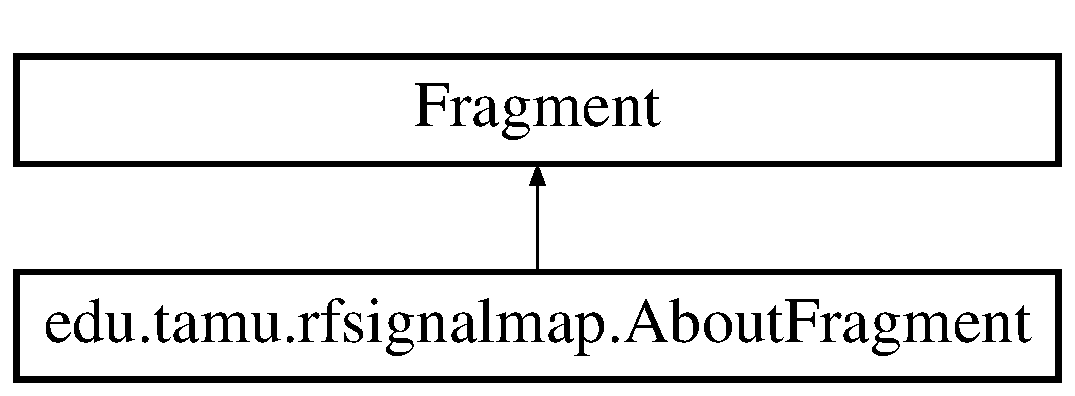
\includegraphics[height=2.000000cm]{classedu_1_1tamu_1_1rfsignalmap_1_1_about_fragment}
\end{center}
\end{figure}
\subsection*{Public Member Functions}
\begin{DoxyCompactItemize}
\item 
void \hyperlink{classedu_1_1tamu_1_1rfsignalmap_1_1_about_fragment_a96b482afac13b664ff351e53633e92af}{on\+Attach} (Context context)
\begin{DoxyCompactList}\small\item\em on\+Attach Event \end{DoxyCompactList}\item 
void \hyperlink{classedu_1_1tamu_1_1rfsignalmap_1_1_about_fragment_a09fd87b64d1d2eea3bc955173fa58308}{on\+Create} (Bundle saved\+Instance\+State)
\begin{DoxyCompactList}\small\item\em on\+Create Event \end{DoxyCompactList}\item 
View \hyperlink{classedu_1_1tamu_1_1rfsignalmap_1_1_about_fragment_aab20df5b3b34cf4f1795f05ec866ee6c}{on\+Create\+View} (Layout\+Inflater inflater, View\+Group parent, Bundle saved\+Instance\+State)
\begin{DoxyCompactList}\small\item\em on\+Create\+View Event \end{DoxyCompactList}\end{DoxyCompactItemize}


\subsection{Detailed Description}
About Fragment -\/ Application Information. 

\subsection{Member Function Documentation}
\index{edu\+::tamu\+::rfsignalmap\+::\+About\+Fragment@{edu\+::tamu\+::rfsignalmap\+::\+About\+Fragment}!on\+Attach@{on\+Attach}}
\index{on\+Attach@{on\+Attach}!edu\+::tamu\+::rfsignalmap\+::\+About\+Fragment@{edu\+::tamu\+::rfsignalmap\+::\+About\+Fragment}}
\subsubsection[{\texorpdfstring{on\+Attach(\+Context context)}{onAttach(Context context)}}]{\setlength{\rightskip}{0pt plus 5cm}edu.\+tamu.\+rfsignalmap.\+About\+Fragment.\+on\+Attach (
\begin{DoxyParamCaption}
\item[{Context}]{context}
\end{DoxyParamCaption}
)}\hypertarget{classedu_1_1tamu_1_1rfsignalmap_1_1_about_fragment_a96b482afac13b664ff351e53633e92af}{}\label{classedu_1_1tamu_1_1rfsignalmap_1_1_about_fragment_a96b482afac13b664ff351e53633e92af}


on\+Attach Event 

Inputs\+: Context Return\+: none Event upon the fragment attaching to the activity \index{edu\+::tamu\+::rfsignalmap\+::\+About\+Fragment@{edu\+::tamu\+::rfsignalmap\+::\+About\+Fragment}!on\+Create@{on\+Create}}
\index{on\+Create@{on\+Create}!edu\+::tamu\+::rfsignalmap\+::\+About\+Fragment@{edu\+::tamu\+::rfsignalmap\+::\+About\+Fragment}}
\subsubsection[{\texorpdfstring{on\+Create(\+Bundle saved\+Instance\+State)}{onCreate(Bundle savedInstanceState)}}]{\setlength{\rightskip}{0pt plus 5cm}edu.\+tamu.\+rfsignalmap.\+About\+Fragment.\+on\+Create (
\begin{DoxyParamCaption}
\item[{Bundle}]{saved\+Instance\+State}
\end{DoxyParamCaption}
)}\hypertarget{classedu_1_1tamu_1_1rfsignalmap_1_1_about_fragment_a09fd87b64d1d2eea3bc955173fa58308}{}\label{classedu_1_1tamu_1_1rfsignalmap_1_1_about_fragment_a09fd87b64d1d2eea3bc955173fa58308}


on\+Create Event 

Inputs\+: Saved Instance State Return\+: none Event on the creation or recreation of this fragment. \index{edu\+::tamu\+::rfsignalmap\+::\+About\+Fragment@{edu\+::tamu\+::rfsignalmap\+::\+About\+Fragment}!on\+Create\+View@{on\+Create\+View}}
\index{on\+Create\+View@{on\+Create\+View}!edu\+::tamu\+::rfsignalmap\+::\+About\+Fragment@{edu\+::tamu\+::rfsignalmap\+::\+About\+Fragment}}
\subsubsection[{\texorpdfstring{on\+Create\+View(\+Layout\+Inflater inflater, View\+Group parent, Bundle saved\+Instance\+State)}{onCreateView(LayoutInflater inflater, ViewGroup parent, Bundle savedInstanceState)}}]{\setlength{\rightskip}{0pt plus 5cm}edu.\+tamu.\+rfsignalmap.\+About\+Fragment.\+on\+Create\+View (
\begin{DoxyParamCaption}
\item[{Layout\+Inflater}]{inflater, }
\item[{View\+Group}]{parent, }
\item[{Bundle}]{saved\+Instance\+State}
\end{DoxyParamCaption}
)}\hypertarget{classedu_1_1tamu_1_1rfsignalmap_1_1_about_fragment_aab20df5b3b34cf4f1795f05ec866ee6c}{}\label{classedu_1_1tamu_1_1rfsignalmap_1_1_about_fragment_aab20df5b3b34cf4f1795f05ec866ee6c}


on\+Create\+View Event 

Inputs\+: Inflater, Container, and Saved Instance State Return\+: View Create View and Fragment Resources 

The documentation for this class was generated from the following file\+:\begin{DoxyCompactItemize}
\item 
app/src/main/java/edu/tamu/rfsignalmap/\hyperlink{_about_fragment_8java}{About\+Fragment.\+java}\end{DoxyCompactItemize}

\hypertarget{classedu_1_1tamu_1_1rfsignalmap_1_1_lat_long}{}\section{edu.\+tamu.\+rfsignalmap.\+Lat\+Long Class Reference}
\label{classedu_1_1tamu_1_1rfsignalmap_1_1_lat_long}\index{edu.\+tamu.\+rfsignalmap.\+Lat\+Long@{edu.\+tamu.\+rfsignalmap.\+Lat\+Long}}


\hyperlink{classedu_1_1tamu_1_1rfsignalmap_1_1_lat_long}{Lat\+Long} class -\/ \hyperlink{classedu_1_1tamu_1_1rfsignalmap_1_1_lat_long}{Lat\+Long} Field Data.  


\subsection*{Public Member Functions}
\begin{DoxyCompactItemize}
\item 
\hyperlink{classedu_1_1tamu_1_1rfsignalmap_1_1_lat_long_aa8531a08ae463ad91b989e553e0d324d}{Lat\+Long} (double azimuth, double distance, double ref\+\_\+lat, double ref\+\_\+long)
\end{DoxyCompactItemize}
\subsection*{Public Attributes}
\begin{DoxyCompactItemize}
\item 
double {\bfseries Latitude}\hypertarget{classedu_1_1tamu_1_1rfsignalmap_1_1_lat_long_aa895c0397b69ff043850188e6b6dc0cb}{}\label{classedu_1_1tamu_1_1rfsignalmap_1_1_lat_long_aa895c0397b69ff043850188e6b6dc0cb}

\item 
double \hyperlink{classedu_1_1tamu_1_1rfsignalmap_1_1_lat_long_ab5440c8a786b2455f09752f89baaf065}{Longitude}\hypertarget{classedu_1_1tamu_1_1rfsignalmap_1_1_lat_long_ab5440c8a786b2455f09752f89baaf065}{}\label{classedu_1_1tamu_1_1rfsignalmap_1_1_lat_long_ab5440c8a786b2455f09752f89baaf065}

\begin{DoxyCompactList}\small\item\em Latitude (as double) \end{DoxyCompactList}\end{DoxyCompactItemize}


\subsection{Detailed Description}
\hyperlink{classedu_1_1tamu_1_1rfsignalmap_1_1_lat_long}{Lat\+Long} class -\/ \hyperlink{classedu_1_1tamu_1_1rfsignalmap_1_1_lat_long}{Lat\+Long} Field Data. 

\subsection{Constructor \& Destructor Documentation}
\index{edu\+::tamu\+::rfsignalmap\+::\+Lat\+Long@{edu\+::tamu\+::rfsignalmap\+::\+Lat\+Long}!Lat\+Long@{Lat\+Long}}
\index{Lat\+Long@{Lat\+Long}!edu\+::tamu\+::rfsignalmap\+::\+Lat\+Long@{edu\+::tamu\+::rfsignalmap\+::\+Lat\+Long}}
\subsubsection[{\texorpdfstring{Lat\+Long(double azimuth, double distance, double ref\+\_\+lat, double ref\+\_\+long)}{LatLong(double azimuth, double distance, double ref_lat, double ref_long)}}]{\setlength{\rightskip}{0pt plus 5cm}edu.\+tamu.\+rfsignalmap.\+Lat\+Long.\+Lat\+Long (
\begin{DoxyParamCaption}
\item[{double}]{azimuth, }
\item[{double}]{distance, }
\item[{double}]{ref\+\_\+lat, }
\item[{double}]{ref\+\_\+long}
\end{DoxyParamCaption}
)}\hypertarget{classedu_1_1tamu_1_1rfsignalmap_1_1_lat_long_aa8531a08ae463ad91b989e553e0d324d}{}\label{classedu_1_1tamu_1_1rfsignalmap_1_1_lat_long_aa8531a08ae463ad91b989e553e0d324d}
Get radian versions

Get distance in meters

Build Sine/\+Cosine values

See Mat Projections Document parameters a \& b

Ellipsoid Radius at Latitude

Build Sine/\+Cosine values of \char`\"{}c\char`\"{}

Covert back to degrees 

The documentation for this class was generated from the following file\+:\begin{DoxyCompactItemize}
\item 
app/src/main/java/edu/tamu/rfsignalmap/\hyperlink{_lat_long_8java}{Lat\+Long.\+java}\end{DoxyCompactItemize}

\hypertarget{classedu_1_1tamu_1_1rfsignalmap_1_1_main_activity}{}\section{edu.\+tamu.\+rfsignalmap.\+Main\+Activity Class Reference}
\label{classedu_1_1tamu_1_1rfsignalmap_1_1_main_activity}\index{edu.\+tamu.\+rfsignalmap.\+Main\+Activity@{edu.\+tamu.\+rfsignalmap.\+Main\+Activity}}


Main Activity Application Project.  


Inheritance diagram for edu.\+tamu.\+rfsignalmap.\+Main\+Activity\+:\begin{figure}[H]
\begin{center}
\leavevmode
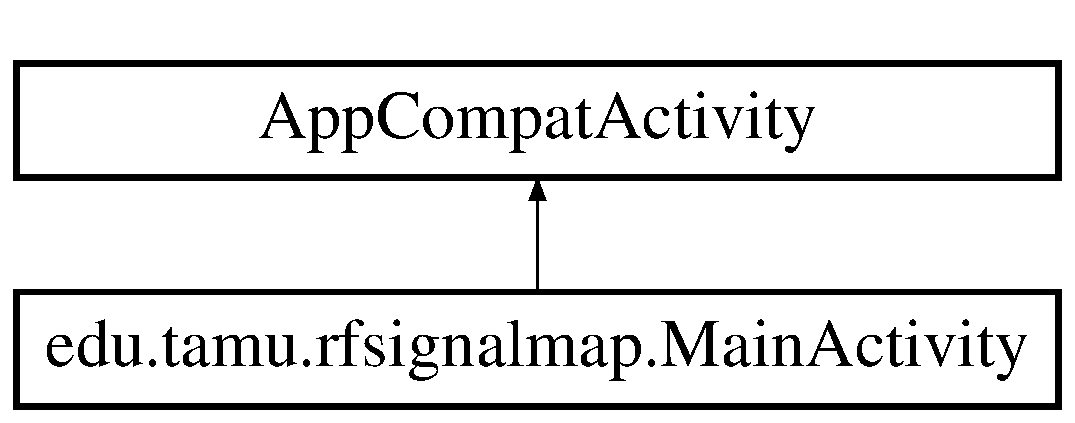
\includegraphics[height=2.000000cm]{classedu_1_1tamu_1_1rfsignalmap_1_1_main_activity}
\end{center}
\end{figure}
\subsection*{Public Member Functions}
\begin{DoxyCompactItemize}
\item 
boolean \hyperlink{classedu_1_1tamu_1_1rfsignalmap_1_1_main_activity_ac14e5eb3ca09daa915b786a6ebfae930}{on\+Create\+Options\+Menu} (Menu menu)
\begin{DoxyCompactList}\small\item\em on\+Create\+Options\+Menu Event \end{DoxyCompactList}\item 
boolean \hyperlink{classedu_1_1tamu_1_1rfsignalmap_1_1_main_activity_a6ccd683ce4cf4baf19105c79124572aa}{on\+Options\+Item\+Selected} (Menu\+Item item)
\begin{DoxyCompactList}\small\item\em on\+Options\+Item\+Selected Event \end{DoxyCompactList}\end{DoxyCompactItemize}
\subsection*{Protected Member Functions}
\begin{DoxyCompactItemize}
\item 
void \hyperlink{classedu_1_1tamu_1_1rfsignalmap_1_1_main_activity_ac8abde5e0a0b83d54d7d8ddaf197b438}{on\+Create} (Bundle saved\+Instance\+State)
\begin{DoxyCompactList}\small\item\em on\+Create Event \end{DoxyCompactList}\end{DoxyCompactItemize}


\subsection{Detailed Description}
Main Activity Application Project. 

\subsection{Member Function Documentation}
\index{edu\+::tamu\+::rfsignalmap\+::\+Main\+Activity@{edu\+::tamu\+::rfsignalmap\+::\+Main\+Activity}!on\+Create@{on\+Create}}
\index{on\+Create@{on\+Create}!edu\+::tamu\+::rfsignalmap\+::\+Main\+Activity@{edu\+::tamu\+::rfsignalmap\+::\+Main\+Activity}}
\subsubsection[{\texorpdfstring{on\+Create(\+Bundle saved\+Instance\+State)}{onCreate(Bundle savedInstanceState)}}]{\setlength{\rightskip}{0pt plus 5cm}edu.\+tamu.\+rfsignalmap.\+Main\+Activity.\+on\+Create (
\begin{DoxyParamCaption}
\item[{Bundle}]{saved\+Instance\+State}
\end{DoxyParamCaption}
)\hspace{0.3cm}{\ttfamily [protected]}}\hypertarget{classedu_1_1tamu_1_1rfsignalmap_1_1_main_activity_ac8abde5e0a0b83d54d7d8ddaf197b438}{}\label{classedu_1_1tamu_1_1rfsignalmap_1_1_main_activity_ac8abde5e0a0b83d54d7d8ddaf197b438}


on\+Create Event 

Inputs\+: saved\+Instance\+State Return\+: none On Create \index{edu\+::tamu\+::rfsignalmap\+::\+Main\+Activity@{edu\+::tamu\+::rfsignalmap\+::\+Main\+Activity}!on\+Create\+Options\+Menu@{on\+Create\+Options\+Menu}}
\index{on\+Create\+Options\+Menu@{on\+Create\+Options\+Menu}!edu\+::tamu\+::rfsignalmap\+::\+Main\+Activity@{edu\+::tamu\+::rfsignalmap\+::\+Main\+Activity}}
\subsubsection[{\texorpdfstring{on\+Create\+Options\+Menu(\+Menu menu)}{onCreateOptionsMenu(Menu menu)}}]{\setlength{\rightskip}{0pt plus 5cm}edu.\+tamu.\+rfsignalmap.\+Main\+Activity.\+on\+Create\+Options\+Menu (
\begin{DoxyParamCaption}
\item[{Menu}]{menu}
\end{DoxyParamCaption}
)}\hypertarget{classedu_1_1tamu_1_1rfsignalmap_1_1_main_activity_ac14e5eb3ca09daa915b786a6ebfae930}{}\label{classedu_1_1tamu_1_1rfsignalmap_1_1_main_activity_ac14e5eb3ca09daa915b786a6ebfae930}


on\+Create\+Options\+Menu Event 

Inputs\+: Menu Return\+: true (boolean) Inflate the menu \index{edu\+::tamu\+::rfsignalmap\+::\+Main\+Activity@{edu\+::tamu\+::rfsignalmap\+::\+Main\+Activity}!on\+Options\+Item\+Selected@{on\+Options\+Item\+Selected}}
\index{on\+Options\+Item\+Selected@{on\+Options\+Item\+Selected}!edu\+::tamu\+::rfsignalmap\+::\+Main\+Activity@{edu\+::tamu\+::rfsignalmap\+::\+Main\+Activity}}
\subsubsection[{\texorpdfstring{on\+Options\+Item\+Selected(\+Menu\+Item item)}{onOptionsItemSelected(MenuItem item)}}]{\setlength{\rightskip}{0pt plus 5cm}edu.\+tamu.\+rfsignalmap.\+Main\+Activity.\+on\+Options\+Item\+Selected (
\begin{DoxyParamCaption}
\item[{Menu\+Item}]{item}
\end{DoxyParamCaption}
)}\hypertarget{classedu_1_1tamu_1_1rfsignalmap_1_1_main_activity_a6ccd683ce4cf4baf19105c79124572aa}{}\label{classedu_1_1tamu_1_1rfsignalmap_1_1_main_activity_a6ccd683ce4cf4baf19105c79124572aa}


on\+Options\+Item\+Selected Event 

Inputs\+: Menu Tem Return\+: true/false (Item is Selected) Perform function based upon menu item selected 

The documentation for this class was generated from the following file\+:\begin{DoxyCompactItemize}
\item 
app/src/main/java/edu/tamu/rfsignalmap/\hyperlink{_main_activity_8java}{Main\+Activity.\+java}\end{DoxyCompactItemize}

\hypertarget{classedu_1_1tamu_1_1rfsignalmap_1_1_main_activity_fragment}{}\section{edu.\+tamu.\+rfsignalmap.\+Main\+Activity\+Fragment Class Reference}
\label{classedu_1_1tamu_1_1rfsignalmap_1_1_main_activity_fragment}\index{edu.\+tamu.\+rfsignalmap.\+Main\+Activity\+Fragment@{edu.\+tamu.\+rfsignalmap.\+Main\+Activity\+Fragment}}


Main Activity Fragment -\/ Display Captured Data.  


Inheritance diagram for edu.\+tamu.\+rfsignalmap.\+Main\+Activity\+Fragment\+:\begin{figure}[H]
\begin{center}
\leavevmode
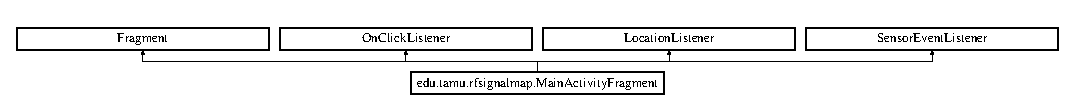
\includegraphics[height=1.048689cm]{classedu_1_1tamu_1_1rfsignalmap_1_1_main_activity_fragment}
\end{center}
\end{figure}
\subsection*{Classes}
\begin{DoxyCompactItemize}
\item 
class {\bfseries Update\+UI}
\begin{DoxyCompactList}\small\item\em User Interface Update from Executor. \end{DoxyCompactList}\end{DoxyCompactItemize}
\subsection*{Public Member Functions}
\begin{DoxyCompactItemize}
\item 
void \hyperlink{classedu_1_1tamu_1_1rfsignalmap_1_1_main_activity_fragment_afa2e497971e51486e7ad03e51e687a24}{on\+Attach} (Context context)
\begin{DoxyCompactList}\small\item\em on\+Attach Event \end{DoxyCompactList}\item 
void \hyperlink{classedu_1_1tamu_1_1rfsignalmap_1_1_main_activity_fragment_a6600a0acb389403f37360350d5a0ddb6}{on\+Create} (Bundle saved\+Instance\+State)
\begin{DoxyCompactList}\small\item\em on\+Create Event \end{DoxyCompactList}\item 
View \hyperlink{classedu_1_1tamu_1_1rfsignalmap_1_1_main_activity_fragment_ac794f6d5686f0644277c3e4e8574e111}{on\+Create\+View} (Layout\+Inflater inflater, View\+Group parent, Bundle saved\+Instance\+State)
\begin{DoxyCompactList}\small\item\em on\+Create\+View Event \end{DoxyCompactList}\item 
void \hyperlink{classedu_1_1tamu_1_1rfsignalmap_1_1_main_activity_fragment_a4205e4271534e663cad10aebf10cd61d}{on\+Stop} ()
\begin{DoxyCompactList}\small\item\em on\+Stop Event \end{DoxyCompactList}\item 
void \hyperlink{classedu_1_1tamu_1_1rfsignalmap_1_1_main_activity_fragment_a7624b00c8e5b8bc595ff3ecca56d3561}{on\+Pause} ()
\begin{DoxyCompactList}\small\item\em on\+Pause Event \end{DoxyCompactList}\item 
void \hyperlink{classedu_1_1tamu_1_1rfsignalmap_1_1_main_activity_fragment_a9341d37b0ffce360a8a403d09d0b2c6b}{on\+Resume} ()
\begin{DoxyCompactList}\small\item\em on\+Resume Event \end{DoxyCompactList}\item 
void \hyperlink{classedu_1_1tamu_1_1rfsignalmap_1_1_main_activity_fragment_a8fc6bd0e569bf3c9a160a22a00d6eb06}{on\+Destroy\+View} ()
\begin{DoxyCompactList}\small\item\em on\+Destroy\+View Event \end{DoxyCompactList}\item 
void \hyperlink{classedu_1_1tamu_1_1rfsignalmap_1_1_main_activity_fragment_ac3f59b7c8c8f3f7547d7d7d1076a75ff}{on\+Destroy} ()
\begin{DoxyCompactList}\small\item\em on\+Destroy Event \end{DoxyCompactList}\item 
void {\bfseries on\+View\+Created} (View view, Bundle saved\+Instance\+State)\hypertarget{classedu_1_1tamu_1_1rfsignalmap_1_1_main_activity_fragment_acffa94c825f2858ede8ea7dd31f3c60e}{}\label{classedu_1_1tamu_1_1rfsignalmap_1_1_main_activity_fragment_acffa94c825f2858ede8ea7dd31f3c60e}

\item 
void \hyperlink{classedu_1_1tamu_1_1rfsignalmap_1_1_main_activity_fragment_a8f2690a0c6e5705769ec4e0534002db5}{on\+Click} (View view)
\begin{DoxyCompactList}\small\item\em on\+Click Event Inputs\+: View Return\+: none Process click events from user \end{DoxyCompactList}\item 
void \hyperlink{classedu_1_1tamu_1_1rfsignalmap_1_1_main_activity_fragment_ab5904b89f6ba8e6b97b513cb17be5194}{on\+Activity\+Created} (Bundle saved\+Instance\+State)\hypertarget{classedu_1_1tamu_1_1rfsignalmap_1_1_main_activity_fragment_ab5904b89f6ba8e6b97b513cb17be5194}{}\label{classedu_1_1tamu_1_1rfsignalmap_1_1_main_activity_fragment_ab5904b89f6ba8e6b97b513cb17be5194}

\begin{DoxyCompactList}\small\item\em on\+Activity\+Created Event Inputs\+: saved\+Instance\+State Return\+: none \end{DoxyCompactList}\item 
void \hyperlink{classedu_1_1tamu_1_1rfsignalmap_1_1_main_activity_fragment_ace61e3e005778db540243ef33e1238e0}{on\+Location\+Changed} (Location location)\hypertarget{classedu_1_1tamu_1_1rfsignalmap_1_1_main_activity_fragment_ace61e3e005778db540243ef33e1238e0}{}\label{classedu_1_1tamu_1_1rfsignalmap_1_1_main_activity_fragment_ace61e3e005778db540243ef33e1238e0}

\begin{DoxyCompactList}\small\item\em on\+Location\+Changed Event Inputs\+: Location Return\+: none Get new Lat/\+Long and assign to current data \end{DoxyCompactList}\item 
void \hyperlink{classedu_1_1tamu_1_1rfsignalmap_1_1_main_activity_fragment_a7411fbbd5dae612d2e3001fbd77c49a1}{on\+Status\+Changed} (String provider, int status, Bundle extras)\hypertarget{classedu_1_1tamu_1_1rfsignalmap_1_1_main_activity_fragment_a7411fbbd5dae612d2e3001fbd77c49a1}{}\label{classedu_1_1tamu_1_1rfsignalmap_1_1_main_activity_fragment_a7411fbbd5dae612d2e3001fbd77c49a1}

\begin{DoxyCompactList}\small\item\em on\+Status\+Changed Event Inputs\+: provider, status, extras Return\+: none Not utilized \end{DoxyCompactList}\item 
void \hyperlink{classedu_1_1tamu_1_1rfsignalmap_1_1_main_activity_fragment_ab8e1fa6c21df3234f821375db06f61f0}{on\+Provider\+Enabled} (String provider)\hypertarget{classedu_1_1tamu_1_1rfsignalmap_1_1_main_activity_fragment_ab8e1fa6c21df3234f821375db06f61f0}{}\label{classedu_1_1tamu_1_1rfsignalmap_1_1_main_activity_fragment_ab8e1fa6c21df3234f821375db06f61f0}

\begin{DoxyCompactList}\small\item\em on\+Provider\+Enabled Event Inputs\+: provider Return\+: none Not utilized \end{DoxyCompactList}\item 
void \hyperlink{classedu_1_1tamu_1_1rfsignalmap_1_1_main_activity_fragment_a2a14a7d8a421c016c748e275d42cd53c}{on\+Provider\+Disabled} (String provider)\hypertarget{classedu_1_1tamu_1_1rfsignalmap_1_1_main_activity_fragment_a2a14a7d8a421c016c748e275d42cd53c}{}\label{classedu_1_1tamu_1_1rfsignalmap_1_1_main_activity_fragment_a2a14a7d8a421c016c748e275d42cd53c}

\begin{DoxyCompactList}\small\item\em on\+Provider\+Disabled Event Not utilized \end{DoxyCompactList}\item 
void \hyperlink{classedu_1_1tamu_1_1rfsignalmap_1_1_main_activity_fragment_a4f905c00c84ac0280a65907957128156}{on\+Sensor\+Changed} (Sensor\+Event event)\hypertarget{classedu_1_1tamu_1_1rfsignalmap_1_1_main_activity_fragment_a4f905c00c84ac0280a65907957128156}{}\label{classedu_1_1tamu_1_1rfsignalmap_1_1_main_activity_fragment_a4f905c00c84ac0280a65907957128156}

\begin{DoxyCompactList}\small\item\em on\+Sensor\+Changed Event Sensor Changes -\/ Get updated data \end{DoxyCompactList}\item 
void \hyperlink{classedu_1_1tamu_1_1rfsignalmap_1_1_main_activity_fragment_ad7c12c1781e31861f91703cb5fef2ee9}{on\+Accuracy\+Changed} (Sensor sensor, int accuracy)\hypertarget{classedu_1_1tamu_1_1rfsignalmap_1_1_main_activity_fragment_ad7c12c1781e31861f91703cb5fef2ee9}{}\label{classedu_1_1tamu_1_1rfsignalmap_1_1_main_activity_fragment_ad7c12c1781e31861f91703cb5fef2ee9}

\begin{DoxyCompactList}\small\item\em Listener not implemented. \end{DoxyCompactList}\end{DoxyCompactItemize}


\subsection{Detailed Description}
Main Activity Fragment -\/ Display Captured Data. 

\subsection{Member Function Documentation}
\index{edu\+::tamu\+::rfsignalmap\+::\+Main\+Activity\+Fragment@{edu\+::tamu\+::rfsignalmap\+::\+Main\+Activity\+Fragment}!on\+Attach@{on\+Attach}}
\index{on\+Attach@{on\+Attach}!edu\+::tamu\+::rfsignalmap\+::\+Main\+Activity\+Fragment@{edu\+::tamu\+::rfsignalmap\+::\+Main\+Activity\+Fragment}}
\subsubsection[{\texorpdfstring{on\+Attach(\+Context context)}{onAttach(Context context)}}]{\setlength{\rightskip}{0pt plus 5cm}void edu.\+tamu.\+rfsignalmap.\+Main\+Activity\+Fragment.\+on\+Attach (
\begin{DoxyParamCaption}
\item[{Context}]{context}
\end{DoxyParamCaption}
)}\hypertarget{classedu_1_1tamu_1_1rfsignalmap_1_1_main_activity_fragment_afa2e497971e51486e7ad03e51e687a24}{}\label{classedu_1_1tamu_1_1rfsignalmap_1_1_main_activity_fragment_afa2e497971e51486e7ad03e51e687a24}


on\+Attach Event 

Inputs\+: none Return\+: none On Attach of Fragment to Context -\/ Fires 1st \index{edu\+::tamu\+::rfsignalmap\+::\+Main\+Activity\+Fragment@{edu\+::tamu\+::rfsignalmap\+::\+Main\+Activity\+Fragment}!on\+Click@{on\+Click}}
\index{on\+Click@{on\+Click}!edu\+::tamu\+::rfsignalmap\+::\+Main\+Activity\+Fragment@{edu\+::tamu\+::rfsignalmap\+::\+Main\+Activity\+Fragment}}
\subsubsection[{\texorpdfstring{on\+Click(\+View view)}{onClick(View view)}}]{\setlength{\rightskip}{0pt plus 5cm}edu.\+tamu.\+rfsignalmap.\+Main\+Activity\+Fragment.\+on\+Click (
\begin{DoxyParamCaption}
\item[{View}]{view}
\end{DoxyParamCaption}
)}\hypertarget{classedu_1_1tamu_1_1rfsignalmap_1_1_main_activity_fragment_a8f2690a0c6e5705769ec4e0534002db5}{}\label{classedu_1_1tamu_1_1rfsignalmap_1_1_main_activity_fragment_a8f2690a0c6e5705769ec4e0534002db5}


on\+Click Event Inputs\+: View Return\+: none Process click events from user 

Process the record button

Disable the button, until finished (from Async task)

Get the current time (sample date / time stamp)

Create a new Async task to save the data

Copy over the data to the class, then execute (will finish in post event) \index{edu\+::tamu\+::rfsignalmap\+::\+Main\+Activity\+Fragment@{edu\+::tamu\+::rfsignalmap\+::\+Main\+Activity\+Fragment}!on\+Create@{on\+Create}}
\index{on\+Create@{on\+Create}!edu\+::tamu\+::rfsignalmap\+::\+Main\+Activity\+Fragment@{edu\+::tamu\+::rfsignalmap\+::\+Main\+Activity\+Fragment}}
\subsubsection[{\texorpdfstring{on\+Create(\+Bundle saved\+Instance\+State)}{onCreate(Bundle savedInstanceState)}}]{\setlength{\rightskip}{0pt plus 5cm}void edu.\+tamu.\+rfsignalmap.\+Main\+Activity\+Fragment.\+on\+Create (
\begin{DoxyParamCaption}
\item[{Bundle}]{saved\+Instance\+State}
\end{DoxyParamCaption}
)}\hypertarget{classedu_1_1tamu_1_1rfsignalmap_1_1_main_activity_fragment_a6600a0acb389403f37360350d5a0ddb6}{}\label{classedu_1_1tamu_1_1rfsignalmap_1_1_main_activity_fragment_a6600a0acb389403f37360350d5a0ddb6}


on\+Create Event 

Inputs\+: Saved Instance State Return\+: none On Creation of Fragment -\/ Fires 2nd Setup scheduled Executor

Open a connection to the first available driver.

Set flag \index{edu\+::tamu\+::rfsignalmap\+::\+Main\+Activity\+Fragment@{edu\+::tamu\+::rfsignalmap\+::\+Main\+Activity\+Fragment}!on\+Create\+View@{on\+Create\+View}}
\index{on\+Create\+View@{on\+Create\+View}!edu\+::tamu\+::rfsignalmap\+::\+Main\+Activity\+Fragment@{edu\+::tamu\+::rfsignalmap\+::\+Main\+Activity\+Fragment}}
\subsubsection[{\texorpdfstring{on\+Create\+View(\+Layout\+Inflater inflater, View\+Group parent, Bundle saved\+Instance\+State)}{onCreateView(LayoutInflater inflater, ViewGroup parent, Bundle savedInstanceState)}}]{\setlength{\rightskip}{0pt plus 5cm}View edu.\+tamu.\+rfsignalmap.\+Main\+Activity\+Fragment.\+on\+Create\+View (
\begin{DoxyParamCaption}
\item[{Layout\+Inflater}]{inflater, }
\item[{View\+Group}]{parent, }
\item[{Bundle}]{saved\+Instance\+State}
\end{DoxyParamCaption}
)}\hypertarget{classedu_1_1tamu_1_1rfsignalmap_1_1_main_activity_fragment_ac794f6d5686f0644277c3e4e8574e111}{}\label{classedu_1_1tamu_1_1rfsignalmap_1_1_main_activity_fragment_ac794f6d5686f0644277c3e4e8574e111}


on\+Create\+View Event 

Inputs\+: Inflater, Container, and Saved Instance State Return\+: View Create View and Fragment Resources \index{edu\+::tamu\+::rfsignalmap\+::\+Main\+Activity\+Fragment@{edu\+::tamu\+::rfsignalmap\+::\+Main\+Activity\+Fragment}!on\+Destroy@{on\+Destroy}}
\index{on\+Destroy@{on\+Destroy}!edu\+::tamu\+::rfsignalmap\+::\+Main\+Activity\+Fragment@{edu\+::tamu\+::rfsignalmap\+::\+Main\+Activity\+Fragment}}
\subsubsection[{\texorpdfstring{on\+Destroy()}{onDestroy()}}]{\setlength{\rightskip}{0pt plus 5cm}edu.\+tamu.\+rfsignalmap.\+Main\+Activity\+Fragment.\+on\+Destroy (
\begin{DoxyParamCaption}
{}
\end{DoxyParamCaption}
)}\hypertarget{classedu_1_1tamu_1_1rfsignalmap_1_1_main_activity_fragment_ac3f59b7c8c8f3f7547d7d7d1076a75ff}{}\label{classedu_1_1tamu_1_1rfsignalmap_1_1_main_activity_fragment_ac3f59b7c8c8f3f7547d7d7d1076a75ff}


on\+Destroy Event 

Inputs\+: none Return\+: none Destroy Event -\/ Close Port Try and close the serial port \index{edu\+::tamu\+::rfsignalmap\+::\+Main\+Activity\+Fragment@{edu\+::tamu\+::rfsignalmap\+::\+Main\+Activity\+Fragment}!on\+Destroy\+View@{on\+Destroy\+View}}
\index{on\+Destroy\+View@{on\+Destroy\+View}!edu\+::tamu\+::rfsignalmap\+::\+Main\+Activity\+Fragment@{edu\+::tamu\+::rfsignalmap\+::\+Main\+Activity\+Fragment}}
\subsubsection[{\texorpdfstring{on\+Destroy\+View()}{onDestroyView()}}]{\setlength{\rightskip}{0pt plus 5cm}edu.\+tamu.\+rfsignalmap.\+Main\+Activity\+Fragment.\+on\+Destroy\+View (
\begin{DoxyParamCaption}
{}
\end{DoxyParamCaption}
)}\hypertarget{classedu_1_1tamu_1_1rfsignalmap_1_1_main_activity_fragment_a8fc6bd0e569bf3c9a160a22a00d6eb06}{}\label{classedu_1_1tamu_1_1rfsignalmap_1_1_main_activity_fragment_a8fc6bd0e569bf3c9a160a22a00d6eb06}


on\+Destroy\+View Event 

Inputs\+: none Return\+: none Destroy View Shutdown the Scheduler, if not already shutdown \index{edu\+::tamu\+::rfsignalmap\+::\+Main\+Activity\+Fragment@{edu\+::tamu\+::rfsignalmap\+::\+Main\+Activity\+Fragment}!on\+Pause@{on\+Pause}}
\index{on\+Pause@{on\+Pause}!edu\+::tamu\+::rfsignalmap\+::\+Main\+Activity\+Fragment@{edu\+::tamu\+::rfsignalmap\+::\+Main\+Activity\+Fragment}}
\subsubsection[{\texorpdfstring{on\+Pause()}{onPause()}}]{\setlength{\rightskip}{0pt plus 5cm}void edu.\+tamu.\+rfsignalmap.\+Main\+Activity\+Fragment.\+on\+Pause (
\begin{DoxyParamCaption}
{}
\end{DoxyParamCaption}
)}\hypertarget{classedu_1_1tamu_1_1rfsignalmap_1_1_main_activity_fragment_a7624b00c8e5b8bc595ff3ecca56d3561}{}\label{classedu_1_1tamu_1_1rfsignalmap_1_1_main_activity_fragment_a7624b00c8e5b8bc595ff3ecca56d3561}


on\+Pause Event 

Inputs\+: none Return\+: none Pause Fragment \index{edu\+::tamu\+::rfsignalmap\+::\+Main\+Activity\+Fragment@{edu\+::tamu\+::rfsignalmap\+::\+Main\+Activity\+Fragment}!on\+Resume@{on\+Resume}}
\index{on\+Resume@{on\+Resume}!edu\+::tamu\+::rfsignalmap\+::\+Main\+Activity\+Fragment@{edu\+::tamu\+::rfsignalmap\+::\+Main\+Activity\+Fragment}}
\subsubsection[{\texorpdfstring{on\+Resume()}{onResume()}}]{\setlength{\rightskip}{0pt plus 5cm}void edu.\+tamu.\+rfsignalmap.\+Main\+Activity\+Fragment.\+on\+Resume (
\begin{DoxyParamCaption}
{}
\end{DoxyParamCaption}
)}\hypertarget{classedu_1_1tamu_1_1rfsignalmap_1_1_main_activity_fragment_a9341d37b0ffce360a8a403d09d0b2c6b}{}\label{classedu_1_1tamu_1_1rfsignalmap_1_1_main_activity_fragment_a9341d37b0ffce360a8a403d09d0b2c6b}


on\+Resume Event 

Inputs\+: none Return\+: none Resume Fragment \index{edu\+::tamu\+::rfsignalmap\+::\+Main\+Activity\+Fragment@{edu\+::tamu\+::rfsignalmap\+::\+Main\+Activity\+Fragment}!on\+Stop@{on\+Stop}}
\index{on\+Stop@{on\+Stop}!edu\+::tamu\+::rfsignalmap\+::\+Main\+Activity\+Fragment@{edu\+::tamu\+::rfsignalmap\+::\+Main\+Activity\+Fragment}}
\subsubsection[{\texorpdfstring{on\+Stop()}{onStop()}}]{\setlength{\rightskip}{0pt plus 5cm}void edu.\+tamu.\+rfsignalmap.\+Main\+Activity\+Fragment.\+on\+Stop (
\begin{DoxyParamCaption}
{}
\end{DoxyParamCaption}
)}\hypertarget{classedu_1_1tamu_1_1rfsignalmap_1_1_main_activity_fragment_a4205e4271534e663cad10aebf10cd61d}{}\label{classedu_1_1tamu_1_1rfsignalmap_1_1_main_activity_fragment_a4205e4271534e663cad10aebf10cd61d}


on\+Stop Event 

Inputs\+: none Return\+: none Stop Fragment 

The documentation for this class was generated from the following file\+:\begin{DoxyCompactItemize}
\item 
app/src/main/java/edu/tamu/rfsignalmap/\hyperlink{_main_activity_fragment_8java}{Main\+Activity\+Fragment.\+java}\end{DoxyCompactItemize}

\hypertarget{classedu_1_1tamu_1_1rfsignalmap_1_1_maps_view_fragment}{}\section{edu.\+tamu.\+rfsignalmap.\+Maps\+View\+Fragment Class Reference}
\label{classedu_1_1tamu_1_1rfsignalmap_1_1_maps_view_fragment}\index{edu.\+tamu.\+rfsignalmap.\+Maps\+View\+Fragment@{edu.\+tamu.\+rfsignalmap.\+Maps\+View\+Fragment}}


Maps View Fragment for Application Project.  


Inheritance diagram for edu.\+tamu.\+rfsignalmap.\+Maps\+View\+Fragment\+:\begin{figure}[H]
\begin{center}
\leavevmode
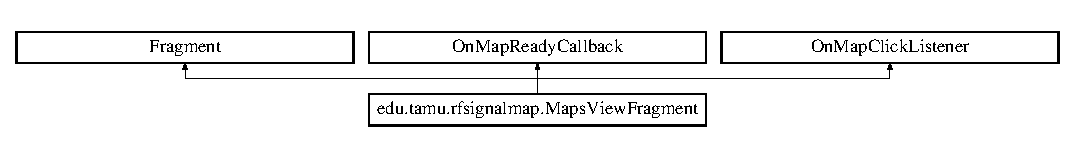
\includegraphics[height=1.458333cm]{classedu_1_1tamu_1_1rfsignalmap_1_1_maps_view_fragment}
\end{center}
\end{figure}
\subsection*{Public Member Functions}
\begin{DoxyCompactItemize}
\item 
void \hyperlink{classedu_1_1tamu_1_1rfsignalmap_1_1_maps_view_fragment_af4d0951688a7b1c3dd8610b80f9e3121}{on\+Attach} (Context context)
\begin{DoxyCompactList}\small\item\em Map Fragment. \end{DoxyCompactList}\item 
void \hyperlink{classedu_1_1tamu_1_1rfsignalmap_1_1_maps_view_fragment_adc896ca074abf84cf2b9d6fc72f8eb85}{on\+Create} (Bundle saved\+Instance\+State)
\begin{DoxyCompactList}\small\item\em on\+Create Event \end{DoxyCompactList}\item 
View \hyperlink{classedu_1_1tamu_1_1rfsignalmap_1_1_maps_view_fragment_a3128669f79328504417a1ae6c87184d2}{on\+Create\+View} (Layout\+Inflater inflater, View\+Group parent, Bundle saved\+Instance\+State)
\begin{DoxyCompactList}\small\item\em on\+Create\+View Event \end{DoxyCompactList}\item 
void \hyperlink{classedu_1_1tamu_1_1rfsignalmap_1_1_maps_view_fragment_a650103568e6ec433aab779ae38c24458}{on\+Map\+Ready} (Google\+Map google\+Map)
\begin{DoxyCompactList}\small\item\em on\+Map\+Ready \end{DoxyCompactList}\item 
void {\bfseries on\+Map\+Click} (Lat\+Lng position)\hypertarget{classedu_1_1tamu_1_1rfsignalmap_1_1_maps_view_fragment_acd9ab237d27dfc41c96bd7cb5ef72ab2}{}\label{classedu_1_1tamu_1_1rfsignalmap_1_1_maps_view_fragment_acd9ab237d27dfc41c96bd7cb5ef72ab2}

\item 
void \hyperlink{classedu_1_1tamu_1_1rfsignalmap_1_1_maps_view_fragment_ab6cfd6c5b2757395c2c71c1e34fe60e1}{Update\+Map} (float Ref\+Latitude, float Ref\+Longitude, float Radius)
\begin{DoxyCompactList}\small\item\em Update\+Map. \end{DoxyCompactList}\end{DoxyCompactItemize}


\subsection{Detailed Description}
Maps View Fragment for Application Project. 

\subsection{Member Function Documentation}
\index{edu\+::tamu\+::rfsignalmap\+::\+Maps\+View\+Fragment@{edu\+::tamu\+::rfsignalmap\+::\+Maps\+View\+Fragment}!on\+Attach@{on\+Attach}}
\index{on\+Attach@{on\+Attach}!edu\+::tamu\+::rfsignalmap\+::\+Maps\+View\+Fragment@{edu\+::tamu\+::rfsignalmap\+::\+Maps\+View\+Fragment}}
\subsubsection[{\texorpdfstring{on\+Attach(\+Context context)}{onAttach(Context context)}}]{\setlength{\rightskip}{0pt plus 5cm}edu.\+tamu.\+rfsignalmap.\+Maps\+View\+Fragment.\+on\+Attach (
\begin{DoxyParamCaption}
\item[{Context}]{context}
\end{DoxyParamCaption}
)}\hypertarget{classedu_1_1tamu_1_1rfsignalmap_1_1_maps_view_fragment_af4d0951688a7b1c3dd8610b80f9e3121}{}\label{classedu_1_1tamu_1_1rfsignalmap_1_1_maps_view_fragment_af4d0951688a7b1c3dd8610b80f9e3121}


Map Fragment. 

on\+Attach Event \begin{DoxyVerb}     Inputs: Context
     Return: none
     Event upon the fragment attaching to the activity\end{DoxyVerb}
 \index{edu\+::tamu\+::rfsignalmap\+::\+Maps\+View\+Fragment@{edu\+::tamu\+::rfsignalmap\+::\+Maps\+View\+Fragment}!on\+Create@{on\+Create}}
\index{on\+Create@{on\+Create}!edu\+::tamu\+::rfsignalmap\+::\+Maps\+View\+Fragment@{edu\+::tamu\+::rfsignalmap\+::\+Maps\+View\+Fragment}}
\subsubsection[{\texorpdfstring{on\+Create(\+Bundle saved\+Instance\+State)}{onCreate(Bundle savedInstanceState)}}]{\setlength{\rightskip}{0pt plus 5cm}edu.\+tamu.\+rfsignalmap.\+Maps\+View\+Fragment.\+on\+Create (
\begin{DoxyParamCaption}
\item[{Bundle}]{saved\+Instance\+State}
\end{DoxyParamCaption}
)}\hypertarget{classedu_1_1tamu_1_1rfsignalmap_1_1_maps_view_fragment_adc896ca074abf84cf2b9d6fc72f8eb85}{}\label{classedu_1_1tamu_1_1rfsignalmap_1_1_maps_view_fragment_adc896ca074abf84cf2b9d6fc72f8eb85}


on\+Create Event 

Inputs\+: Saved Instance State Return\+: none Event on the creation or recreation of this fragment. \index{edu\+::tamu\+::rfsignalmap\+::\+Maps\+View\+Fragment@{edu\+::tamu\+::rfsignalmap\+::\+Maps\+View\+Fragment}!on\+Create\+View@{on\+Create\+View}}
\index{on\+Create\+View@{on\+Create\+View}!edu\+::tamu\+::rfsignalmap\+::\+Maps\+View\+Fragment@{edu\+::tamu\+::rfsignalmap\+::\+Maps\+View\+Fragment}}
\subsubsection[{\texorpdfstring{on\+Create\+View(\+Layout\+Inflater inflater, View\+Group parent, Bundle saved\+Instance\+State)}{onCreateView(LayoutInflater inflater, ViewGroup parent, Bundle savedInstanceState)}}]{\setlength{\rightskip}{0pt plus 5cm}edu.\+tamu.\+rfsignalmap.\+Maps\+View\+Fragment.\+on\+Create\+View (
\begin{DoxyParamCaption}
\item[{Layout\+Inflater}]{inflater, }
\item[{View\+Group}]{parent, }
\item[{Bundle}]{saved\+Instance\+State}
\end{DoxyParamCaption}
)}\hypertarget{classedu_1_1tamu_1_1rfsignalmap_1_1_maps_view_fragment_a3128669f79328504417a1ae6c87184d2}{}\label{classedu_1_1tamu_1_1rfsignalmap_1_1_maps_view_fragment_a3128669f79328504417a1ae6c87184d2}


on\+Create\+View Event 

Inputs\+: saved\+Instance\+State Return\+: View Create View and Fragment Resources \index{edu\+::tamu\+::rfsignalmap\+::\+Maps\+View\+Fragment@{edu\+::tamu\+::rfsignalmap\+::\+Maps\+View\+Fragment}!on\+Map\+Ready@{on\+Map\+Ready}}
\index{on\+Map\+Ready@{on\+Map\+Ready}!edu\+::tamu\+::rfsignalmap\+::\+Maps\+View\+Fragment@{edu\+::tamu\+::rfsignalmap\+::\+Maps\+View\+Fragment}}
\subsubsection[{\texorpdfstring{on\+Map\+Ready(\+Google\+Map google\+Map)}{onMapReady(GoogleMap googleMap)}}]{\setlength{\rightskip}{0pt plus 5cm}edu.\+tamu.\+rfsignalmap.\+Maps\+View\+Fragment.\+on\+Map\+Ready (
\begin{DoxyParamCaption}
\item[{Google\+Map}]{google\+Map}
\end{DoxyParamCaption}
)}\hypertarget{classedu_1_1tamu_1_1rfsignalmap_1_1_maps_view_fragment_a650103568e6ec433aab779ae38c24458}{}\label{classedu_1_1tamu_1_1rfsignalmap_1_1_maps_view_fragment_a650103568e6ec433aab779ae38c24458}


on\+Map\+Ready 

Inputs\+: google\+Map Return\+: none Manipulates the map once available. This callback is triggered when the map is ready to be used. Get the map now that it is ready

Add a marker in E\+IC and move the camera We will need to hack this to work with other lat/long values to be displayed \index{edu\+::tamu\+::rfsignalmap\+::\+Maps\+View\+Fragment@{edu\+::tamu\+::rfsignalmap\+::\+Maps\+View\+Fragment}!Update\+Map@{Update\+Map}}
\index{Update\+Map@{Update\+Map}!edu\+::tamu\+::rfsignalmap\+::\+Maps\+View\+Fragment@{edu\+::tamu\+::rfsignalmap\+::\+Maps\+View\+Fragment}}
\subsubsection[{\texorpdfstring{Update\+Map(float Ref\+Latitude, float Ref\+Longitude, float Radius)}{UpdateMap(float RefLatitude, float RefLongitude, float Radius)}}]{\setlength{\rightskip}{0pt plus 5cm}edu.\+tamu.\+rfsignalmap.\+Maps\+View\+Fragment.\+Update\+Map (
\begin{DoxyParamCaption}
\item[{float}]{Ref\+Latitude, }
\item[{float}]{Ref\+Longitude, }
\item[{float}]{Radius}
\end{DoxyParamCaption}
)}\hypertarget{classedu_1_1tamu_1_1rfsignalmap_1_1_maps_view_fragment_ab6cfd6c5b2757395c2c71c1e34fe60e1}{}\label{classedu_1_1tamu_1_1rfsignalmap_1_1_maps_view_fragment_ab6cfd6c5b2757395c2c71c1e34fe60e1}


Update\+Map. 

Iputs\+: Center location (Lat/\+Long), Radius to get data from reference Return\+: none Manipulates the map once available and gets the data from the database 

The documentation for this class was generated from the following file\+:\begin{DoxyCompactItemize}
\item 
app/src/main/java/edu/tamu/rfsignalmap/Maps\+View\+Fragment.\+java\end{DoxyCompactItemize}

\hypertarget{classedu_1_1tamu_1_1rfsignalmap_1_1_r_f_data}{}\section{edu.\+tamu.\+rfsignalmap.\+R\+F\+Data Class Reference}
\label{classedu_1_1tamu_1_1rfsignalmap_1_1_r_f_data}\index{edu.\+tamu.\+rfsignalmap.\+R\+F\+Data@{edu.\+tamu.\+rfsignalmap.\+R\+F\+Data}}


\hyperlink{classedu_1_1tamu_1_1rfsignalmap_1_1_r_f_data}{R\+F\+Data} class -\/ RF Field Data w/ J\+S\+ON support.  


\subsection*{Public Member Functions}
\begin{DoxyCompactItemize}
\item 
\hyperlink{classedu_1_1tamu_1_1rfsignalmap_1_1_r_f_data_a4e1a112c9551e41c445c79c94bf394c2}{R\+F\+Data} ()
\begin{DoxyCompactList}\small\item\em \hyperlink{classedu_1_1tamu_1_1rfsignalmap_1_1_r_f_data}{R\+F\+Data} -\/ Constructor. \end{DoxyCompactList}\end{DoxyCompactItemize}
\subsection*{Public Attributes}
\begin{DoxyCompactItemize}
\item 
int {\bfseries Sample\+Number}\hypertarget{classedu_1_1tamu_1_1rfsignalmap_1_1_r_f_data_a972c6f020329c70b4e27ab49b6b5ced2}{}\label{classedu_1_1tamu_1_1rfsignalmap_1_1_r_f_data_a972c6f020329c70b4e27ab49b6b5ced2}

\item 
int {\bfseries Xbee\+ID}\hypertarget{classedu_1_1tamu_1_1rfsignalmap_1_1_r_f_data_a2b06dff84b63a25814421edbcd422aae}{}\label{classedu_1_1tamu_1_1rfsignalmap_1_1_r_f_data_a2b06dff84b63a25814421edbcd422aae}

\item 
int {\bfseries Device\+ID}\hypertarget{classedu_1_1tamu_1_1rfsignalmap_1_1_r_f_data_aece0edbefbc573116884957c3f9a4f6e}{}\label{classedu_1_1tamu_1_1rfsignalmap_1_1_r_f_data_aece0edbefbc573116884957c3f9a4f6e}

\item 
double {\bfseries R\+S\+SI}\hypertarget{classedu_1_1tamu_1_1rfsignalmap_1_1_r_f_data_afbefa9e948b35a2b6fe5e6a52c4b7d10}{}\label{classedu_1_1tamu_1_1rfsignalmap_1_1_r_f_data_afbefa9e948b35a2b6fe5e6a52c4b7d10}

\item 
String {\bfseries Cell\+Signal\+Strength}\hypertarget{classedu_1_1tamu_1_1rfsignalmap_1_1_r_f_data_a341376c51f2ccad5f62f69b34c5f1898}{}\label{classedu_1_1tamu_1_1rfsignalmap_1_1_r_f_data_a341376c51f2ccad5f62f69b34c5f1898}

\item 
double {\bfseries Latitude}\hypertarget{classedu_1_1tamu_1_1rfsignalmap_1_1_r_f_data_a33961aa8f213adfc213770dc5a88066e}{}\label{classedu_1_1tamu_1_1rfsignalmap_1_1_r_f_data_a33961aa8f213adfc213770dc5a88066e}

\item 
double {\bfseries Longitude}\hypertarget{classedu_1_1tamu_1_1rfsignalmap_1_1_r_f_data_a238802176504158d4285ed57f57ebcbf}{}\label{classedu_1_1tamu_1_1rfsignalmap_1_1_r_f_data_a238802176504158d4285ed57f57ebcbf}

\item 
double {\bfseries Yaw}\hypertarget{classedu_1_1tamu_1_1rfsignalmap_1_1_r_f_data_ada19ec18608fd3461c7ed202ef2c64a4}{}\label{classedu_1_1tamu_1_1rfsignalmap_1_1_r_f_data_ada19ec18608fd3461c7ed202ef2c64a4}

\item 
double {\bfseries Pitch}\hypertarget{classedu_1_1tamu_1_1rfsignalmap_1_1_r_f_data_a8d4fb317f4c44567b4bb1abf72fa0a69}{}\label{classedu_1_1tamu_1_1rfsignalmap_1_1_r_f_data_a8d4fb317f4c44567b4bb1abf72fa0a69}

\item 
double {\bfseries Roll}\hypertarget{classedu_1_1tamu_1_1rfsignalmap_1_1_r_f_data_aa9fc218c116f1b97b655177fa7511057}{}\label{classedu_1_1tamu_1_1rfsignalmap_1_1_r_f_data_aa9fc218c116f1b97b655177fa7511057}

\item 
Date {\bfseries Sample\+Date}\hypertarget{classedu_1_1tamu_1_1rfsignalmap_1_1_r_f_data_a321c28e1d0182ad8e62c7c590acb31d2}{}\label{classedu_1_1tamu_1_1rfsignalmap_1_1_r_f_data_a321c28e1d0182ad8e62c7c590acb31d2}

\end{DoxyCompactItemize}


\subsection{Detailed Description}
\hyperlink{classedu_1_1tamu_1_1rfsignalmap_1_1_r_f_data}{R\+F\+Data} class -\/ RF Field Data w/ J\+S\+ON support. 

\subsection{Constructor \& Destructor Documentation}
\index{edu\+::tamu\+::rfsignalmap\+::\+R\+F\+Data@{edu\+::tamu\+::rfsignalmap\+::\+R\+F\+Data}!R\+F\+Data@{R\+F\+Data}}
\index{R\+F\+Data@{R\+F\+Data}!edu\+::tamu\+::rfsignalmap\+::\+R\+F\+Data@{edu\+::tamu\+::rfsignalmap\+::\+R\+F\+Data}}
\subsubsection[{\texorpdfstring{R\+F\+Data()}{RFData()}}]{\setlength{\rightskip}{0pt plus 5cm}edu.\+tamu.\+rfsignalmap.\+R\+F\+Data.\+R\+F\+Data (
\begin{DoxyParamCaption}
{}
\end{DoxyParamCaption}
)}\hypertarget{classedu_1_1tamu_1_1rfsignalmap_1_1_r_f_data_a4e1a112c9551e41c445c79c94bf394c2}{}\label{classedu_1_1tamu_1_1rfsignalmap_1_1_r_f_data_a4e1a112c9551e41c445c79c94bf394c2}


\hyperlink{classedu_1_1tamu_1_1rfsignalmap_1_1_r_f_data}{R\+F\+Data} -\/ Constructor. 

\hyperlink{classedu_1_1tamu_1_1rfsignalmap_1_1_r_f_data}{R\+F\+Data}, no initialization given, just set defaults Default is -\/1 (undefined)

Default is -\/1 (undefined)

Default is -\/1 (undefined) 

The documentation for this class was generated from the following file\+:\begin{DoxyCompactItemize}
\item 
app/src/main/java/edu/tamu/rfsignalmap/\hyperlink{_r_f_data_8java}{R\+F\+Data.\+java}\end{DoxyCompactItemize}

\hypertarget{classedu_1_1tamu_1_1rfsignalmap_1_1_r_f_field_s_q_l_database}{}\section{edu.\+tamu.\+rfsignalmap.\+R\+F\+Field\+S\+Q\+L\+Database Class Reference}
\label{classedu_1_1tamu_1_1rfsignalmap_1_1_r_f_field_s_q_l_database}\index{edu.\+tamu.\+rfsignalmap.\+R\+F\+Field\+S\+Q\+L\+Database@{edu.\+tamu.\+rfsignalmap.\+R\+F\+Field\+S\+Q\+L\+Database}}


\hyperlink{classedu_1_1tamu_1_1rfsignalmap_1_1_r_f_field_s_q_l_database}{R\+F\+Field\+S\+Q\+L\+Database} interfaces S\+QL Database, supplies methods to access data and passes.  


\subsection*{Public Member Functions}
\begin{DoxyCompactItemize}
\item 
\hyperlink{classedu_1_1tamu_1_1rfsignalmap_1_1_r_f_field_s_q_l_database_a3ec094dfb43ac20c47c9544f236c23f6}{R\+F\+Field\+S\+Q\+L\+Database} ()
\begin{DoxyCompactList}\small\item\em My\+Sql Database connection. \end{DoxyCompactList}\item 
boolean \hyperlink{classedu_1_1tamu_1_1rfsignalmap_1_1_r_f_field_s_q_l_database_a410c5236687fb8cdb8ae422f675a1149}{Connect\+To\+Database} (String host\+\_\+address)
\begin{DoxyCompactList}\small\item\em Connect\+To\+Database. \end{DoxyCompactList}\item 
boolean \hyperlink{classedu_1_1tamu_1_1rfsignalmap_1_1_r_f_field_s_q_l_database_a4144f9565e37492fe3f674821f89bea8}{Disconnect\+Database} ()
\begin{DoxyCompactList}\small\item\em Disconnect\+Database. \end{DoxyCompactList}\item 
boolean \hyperlink{classedu_1_1tamu_1_1rfsignalmap_1_1_r_f_field_s_q_l_database_ae74d741116f0f986f6f4a293b484b0f3}{Add\+New\+Entry} (\hyperlink{classedu_1_1tamu_1_1rfsignalmap_1_1_r_f_data}{R\+F\+Data} R\+F\+Member)
\begin{DoxyCompactList}\small\item\em Add\+New\+Entry. \end{DoxyCompactList}\item 
Array\+List \hyperlink{classedu_1_1tamu_1_1rfsignalmap_1_1_r_f_field_s_q_l_database_a0be5bce356ff7106cc96686e3946a2c3}{List\+Data\+By\+Geo\+Area} (float Start\+Latitude, float Start\+Longitude, float End\+Latitude, float End\+Longitude)
\begin{DoxyCompactList}\small\item\em List\+Data\+By\+Geo\+Area. \end{DoxyCompactList}\end{DoxyCompactItemize}


\subsection{Detailed Description}
\hyperlink{classedu_1_1tamu_1_1rfsignalmap_1_1_r_f_field_s_q_l_database}{R\+F\+Field\+S\+Q\+L\+Database} interfaces S\+QL Database, supplies methods to access data and passes. 

\subsection{Constructor \& Destructor Documentation}
\index{edu\+::tamu\+::rfsignalmap\+::\+R\+F\+Field\+S\+Q\+L\+Database@{edu\+::tamu\+::rfsignalmap\+::\+R\+F\+Field\+S\+Q\+L\+Database}!R\+F\+Field\+S\+Q\+L\+Database@{R\+F\+Field\+S\+Q\+L\+Database}}
\index{R\+F\+Field\+S\+Q\+L\+Database@{R\+F\+Field\+S\+Q\+L\+Database}!edu\+::tamu\+::rfsignalmap\+::\+R\+F\+Field\+S\+Q\+L\+Database@{edu\+::tamu\+::rfsignalmap\+::\+R\+F\+Field\+S\+Q\+L\+Database}}
\subsubsection[{\texorpdfstring{R\+F\+Field\+S\+Q\+L\+Database()}{RFFieldSQLDatabase()}}]{\setlength{\rightskip}{0pt plus 5cm}edu.\+tamu.\+rfsignalmap.\+R\+F\+Field\+S\+Q\+L\+Database.\+R\+F\+Field\+S\+Q\+L\+Database (
\begin{DoxyParamCaption}
{}
\end{DoxyParamCaption}
)}\hypertarget{classedu_1_1tamu_1_1rfsignalmap_1_1_r_f_field_s_q_l_database_a3ec094dfb43ac20c47c9544f236c23f6}{}\label{classedu_1_1tamu_1_1rfsignalmap_1_1_r_f_field_s_q_l_database_a3ec094dfb43ac20c47c9544f236c23f6}


My\+Sql Database connection. 

\hyperlink{classedu_1_1tamu_1_1rfsignalmap_1_1_r_f_field_s_q_l_database}{R\+F\+Field\+S\+Q\+L\+Database} -\/ Constructor \begin{DoxyVerb}     RFFieldSQLDatabase, no initialization given\end{DoxyVerb}
 

\subsection{Member Function Documentation}
\index{edu\+::tamu\+::rfsignalmap\+::\+R\+F\+Field\+S\+Q\+L\+Database@{edu\+::tamu\+::rfsignalmap\+::\+R\+F\+Field\+S\+Q\+L\+Database}!Add\+New\+Entry@{Add\+New\+Entry}}
\index{Add\+New\+Entry@{Add\+New\+Entry}!edu\+::tamu\+::rfsignalmap\+::\+R\+F\+Field\+S\+Q\+L\+Database@{edu\+::tamu\+::rfsignalmap\+::\+R\+F\+Field\+S\+Q\+L\+Database}}
\subsubsection[{\texorpdfstring{Add\+New\+Entry(\+R\+F\+Data R\+F\+Member)}{AddNewEntry(RFData RFMember)}}]{\setlength{\rightskip}{0pt plus 5cm}edu.\+tamu.\+rfsignalmap.\+R\+F\+Field\+S\+Q\+L\+Database.\+Add\+New\+Entry (
\begin{DoxyParamCaption}
\item[{{\bf R\+F\+Data}}]{R\+F\+Member}
\end{DoxyParamCaption}
)}\hypertarget{classedu_1_1tamu_1_1rfsignalmap_1_1_r_f_field_s_q_l_database_ae74d741116f0f986f6f4a293b484b0f3}{}\label{classedu_1_1tamu_1_1rfsignalmap_1_1_r_f_field_s_q_l_database_ae74d741116f0f986f6f4a293b484b0f3}


Add\+New\+Entry. 

Inputs\+: RF Data Entry Return\+: Success = T\+R\+UE / Failure = F\+A\+L\+SE Insert new data to table (executes S\+QL command) Return status (success / failure)

Try to get J\+S\+ON, and save data to database

If not default then save data

Build up S\+QL string

Insert S\+QL statement, Table\+: R\+F\+\_\+\+Fields

Field\+: int\+Xbee\+ID

Field\+: int\+Device\+ID

Field\+: flt\+R\+S\+SI

Field\+: flt\+Latitude

Field\+: flt\+Longitude

Field\+: flt\+Yaw

Field\+: flt\+Pitch

Field\+: flt\+Roll

Field\+: txt\+Cell\+Signal\+Strength

Field\+: dt\+Sample\+Date

Values indetifier

Value\+: Xbee\+ID

Value\+: Device\+ID

Value\+: R\+S\+SI

Value\+: Latitude

Value\+: Longitude

Value\+: Yaw

Value\+: Pitch

Value\+: Roll

Value\+: Cell\+Signal\+Strength

Debug print the S\+QL statement

Build S\+QL statement

Execute the S\+QL statement

Close the statement

Success

Print the exception data and exit

Failure, invalid J\+S\+ON or data

Exception processing\+:

Print the exception data and exit

Failure

Return status \index{edu\+::tamu\+::rfsignalmap\+::\+R\+F\+Field\+S\+Q\+L\+Database@{edu\+::tamu\+::rfsignalmap\+::\+R\+F\+Field\+S\+Q\+L\+Database}!Connect\+To\+Database@{Connect\+To\+Database}}
\index{Connect\+To\+Database@{Connect\+To\+Database}!edu\+::tamu\+::rfsignalmap\+::\+R\+F\+Field\+S\+Q\+L\+Database@{edu\+::tamu\+::rfsignalmap\+::\+R\+F\+Field\+S\+Q\+L\+Database}}
\subsubsection[{\texorpdfstring{Connect\+To\+Database(\+String host\+\_\+address)}{ConnectToDatabase(String host_address)}}]{\setlength{\rightskip}{0pt plus 5cm}edu.\+tamu.\+rfsignalmap.\+R\+F\+Field\+S\+Q\+L\+Database.\+Connect\+To\+Database (
\begin{DoxyParamCaption}
\item[{String}]{host\+\_\+address}
\end{DoxyParamCaption}
)}\hypertarget{classedu_1_1tamu_1_1rfsignalmap_1_1_r_f_field_s_q_l_database_a410c5236687fb8cdb8ae422f675a1149}{}\label{classedu_1_1tamu_1_1rfsignalmap_1_1_r_f_field_s_q_l_database_a410c5236687fb8cdb8ae422f675a1149}


Connect\+To\+Database. 

Inputs\+: host address for server, username, password Return\+: Success = T\+R\+UE / Failure = F\+A\+L\+SE Establishes a connection to the database Return status (success / failure)

Try and connect to the My\+S\+QL Database

Use E\+C\+E\+N\+\_\+\+R\+F\+\_\+\+Field Database

Print out connection success

Print out connection success

Success

Exception processing\+:

Print the exception data and exit

Failure

Return status \index{edu\+::tamu\+::rfsignalmap\+::\+R\+F\+Field\+S\+Q\+L\+Database@{edu\+::tamu\+::rfsignalmap\+::\+R\+F\+Field\+S\+Q\+L\+Database}!Disconnect\+Database@{Disconnect\+Database}}
\index{Disconnect\+Database@{Disconnect\+Database}!edu\+::tamu\+::rfsignalmap\+::\+R\+F\+Field\+S\+Q\+L\+Database@{edu\+::tamu\+::rfsignalmap\+::\+R\+F\+Field\+S\+Q\+L\+Database}}
\subsubsection[{\texorpdfstring{Disconnect\+Database()}{DisconnectDatabase()}}]{\setlength{\rightskip}{0pt plus 5cm}edu.\+tamu.\+rfsignalmap.\+R\+F\+Field\+S\+Q\+L\+Database.\+Disconnect\+Database (
\begin{DoxyParamCaption}
{}
\end{DoxyParamCaption}
)}\hypertarget{classedu_1_1tamu_1_1rfsignalmap_1_1_r_f_field_s_q_l_database_a4144f9565e37492fe3f674821f89bea8}{}\label{classedu_1_1tamu_1_1rfsignalmap_1_1_r_f_field_s_q_l_database_a4144f9565e37492fe3f674821f89bea8}


Disconnect\+Database. 

Inputs\+: none Return\+: Success = T\+R\+UE / Failure = F\+A\+L\+SE Disconnects the connection to the database Return status (success / failure)

Try and connect to the My\+S\+QL Database

Close the connection if defined

Print out status

Success

Exception processing\+:

Print the exception data and exit

Failure

Return status \index{edu\+::tamu\+::rfsignalmap\+::\+R\+F\+Field\+S\+Q\+L\+Database@{edu\+::tamu\+::rfsignalmap\+::\+R\+F\+Field\+S\+Q\+L\+Database}!List\+Data\+By\+Geo\+Area@{List\+Data\+By\+Geo\+Area}}
\index{List\+Data\+By\+Geo\+Area@{List\+Data\+By\+Geo\+Area}!edu\+::tamu\+::rfsignalmap\+::\+R\+F\+Field\+S\+Q\+L\+Database@{edu\+::tamu\+::rfsignalmap\+::\+R\+F\+Field\+S\+Q\+L\+Database}}
\subsubsection[{\texorpdfstring{List\+Data\+By\+Geo\+Area(float Start\+Latitude, float Start\+Longitude, float End\+Latitude, float End\+Longitude)}{ListDataByGeoArea(float StartLatitude, float StartLongitude, float EndLatitude, float EndLongitude)}}]{\setlength{\rightskip}{0pt plus 5cm}edu.\+tamu.\+rfsignalmap.\+R\+F\+Field\+S\+Q\+L\+Database.\+List\+Data\+By\+Geo\+Area (
\begin{DoxyParamCaption}
\item[{float}]{Start\+Latitude, }
\item[{float}]{Start\+Longitude, }
\item[{float}]{End\+Latitude, }
\item[{float}]{End\+Longitude}
\end{DoxyParamCaption}
)}\hypertarget{classedu_1_1tamu_1_1rfsignalmap_1_1_r_f_field_s_q_l_database_a0be5bce356ff7106cc96686e3946a2c3}{}\label{classedu_1_1tamu_1_1rfsignalmap_1_1_r_f_field_s_q_l_database_a0be5bce356ff7106cc96686e3946a2c3}


List\+Data\+By\+Geo\+Area. 

Inputs\+: Start Latitude, Start Longitude, End Latitude, End Longitude (create rectangle) Return\+: RF Data Entryies (Array\+List) Get RF Data Entries given Geo Constraints Print debug information to port

Build up S\+QL string

Select S\+QL statement

Field\+: int\+Sample\+Num

Field\+: int\+Xbee\+ID

Field\+: int\+Device\+ID

Field\+: flt\+R\+S\+SI

Field\+: flt\+Latitude

Field\+: flt\+Longitude

Field\+: flt\+Yaw

Field\+: flt\+Pitch

Field\+: flt\+Roll

Field\+: txt\+Cell\+Signal\+Strength

Field\+: dt\+Sample\+Date

Table\+: R\+F\+\_\+\+Fields

If, 0,0,0,0 return all records

Where statement

Field on Where and condition

Field on Where and condition

Field on Where and condition

Field on Where and condition

Debug print the S\+QL statement

Build S\+QL statement

Execute the S\+QL statement as a query

Read the records

Close the record set

Close the statement

If empty then print out no records found

Print the fact that no record was found

Exception processing\+:

Print the exception data and exit

Return Record Set 

The documentation for this class was generated from the following file\+:\begin{DoxyCompactItemize}
\item 
app/src/main/java/edu/tamu/rfsignalmap/\hyperlink{_r_f_field_s_q_l_database_8java}{R\+F\+Field\+S\+Q\+L\+Database.\+java}\end{DoxyCompactItemize}

\hypertarget{classedu_1_1tamu_1_1rfsignalmap_1_1_settings_fragment}{}\section{edu.\+tamu.\+rfsignalmap.\+Settings\+Fragment Class Reference}
\label{classedu_1_1tamu_1_1rfsignalmap_1_1_settings_fragment}\index{edu.\+tamu.\+rfsignalmap.\+Settings\+Fragment@{edu.\+tamu.\+rfsignalmap.\+Settings\+Fragment}}


Settings Fragment -\/ Application Information.  


Inheritance diagram for edu.\+tamu.\+rfsignalmap.\+Settings\+Fragment\+:\begin{figure}[H]
\begin{center}
\leavevmode
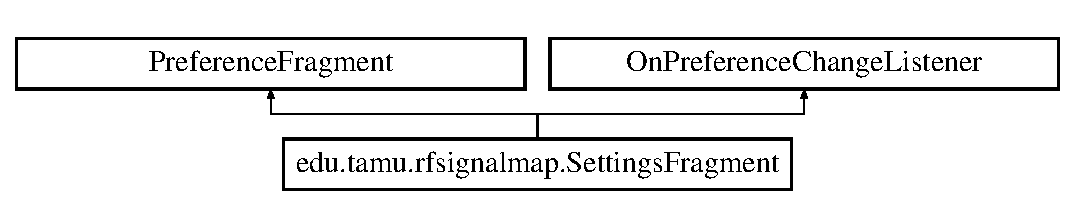
\includegraphics[height=2.000000cm]{classedu_1_1tamu_1_1rfsignalmap_1_1_settings_fragment}
\end{center}
\end{figure}
\subsection*{Public Member Functions}
\begin{DoxyCompactItemize}
\item 
void {\bfseries on\+Attach} (Context context)\hypertarget{classedu_1_1tamu_1_1rfsignalmap_1_1_settings_fragment_aadf43016ef135a1e5169e998d5b8ff83}{}\label{classedu_1_1tamu_1_1rfsignalmap_1_1_settings_fragment_aadf43016ef135a1e5169e998d5b8ff83}

\item 
void {\bfseries on\+Create} (Bundle saved\+Instance\+State)\hypertarget{classedu_1_1tamu_1_1rfsignalmap_1_1_settings_fragment_aff3f72f2aa6dbb4cd10e6d614aae8287}{}\label{classedu_1_1tamu_1_1rfsignalmap_1_1_settings_fragment_aff3f72f2aa6dbb4cd10e6d614aae8287}

\item 
View \hyperlink{classedu_1_1tamu_1_1rfsignalmap_1_1_settings_fragment_a1dc3057a7372763d9499a2a38b5dc339}{on\+Create\+View} (Layout\+Inflater inflater, View\+Group parent, Bundle saved\+Instance\+State)
\begin{DoxyCompactList}\small\item\em on\+Create\+View Event \end{DoxyCompactList}\item 
void {\bfseries on\+View\+Created} (View view, Bundle saved\+Instance\+State)\hypertarget{classedu_1_1tamu_1_1rfsignalmap_1_1_settings_fragment_aa9cdfb48cdf85edaca43117131934646}{}\label{classedu_1_1tamu_1_1rfsignalmap_1_1_settings_fragment_aa9cdfb48cdf85edaca43117131934646}

\item 
void {\bfseries on\+Activity\+Created} (Bundle saved\+Instance\+State)\hypertarget{classedu_1_1tamu_1_1rfsignalmap_1_1_settings_fragment_afd602256dd19948e343575c5a0924c09}{}\label{classedu_1_1tamu_1_1rfsignalmap_1_1_settings_fragment_afd602256dd19948e343575c5a0924c09}

\item 
void \hyperlink{classedu_1_1tamu_1_1rfsignalmap_1_1_settings_fragment_abd35754f99cbb57ae98a596d96265133}{on\+Start} ()\hypertarget{classedu_1_1tamu_1_1rfsignalmap_1_1_settings_fragment_abd35754f99cbb57ae98a596d96265133}{}\label{classedu_1_1tamu_1_1rfsignalmap_1_1_settings_fragment_abd35754f99cbb57ae98a596d96265133}

\begin{DoxyCompactList}\small\item\em Get server settings and display them. \end{DoxyCompactList}\item 
boolean \hyperlink{classedu_1_1tamu_1_1rfsignalmap_1_1_settings_fragment_ac8251b6f76caa8443e6585c3e2fd8ed4}{on\+Preference\+Change} (Preference preference, Object new\+Value)\hypertarget{classedu_1_1tamu_1_1rfsignalmap_1_1_settings_fragment_ac8251b6f76caa8443e6585c3e2fd8ed4}{}\label{classedu_1_1tamu_1_1rfsignalmap_1_1_settings_fragment_ac8251b6f76caa8443e6585c3e2fd8ed4}

\begin{DoxyCompactList}\small\item\em This method is invoked whenever a change has been made to any of the settings items. \end{DoxyCompactList}\end{DoxyCompactItemize}


\subsection{Detailed Description}
Settings Fragment -\/ Application Information. 

\subsection{Member Function Documentation}
\index{edu\+::tamu\+::rfsignalmap\+::\+Settings\+Fragment@{edu\+::tamu\+::rfsignalmap\+::\+Settings\+Fragment}!on\+Create\+View@{on\+Create\+View}}
\index{on\+Create\+View@{on\+Create\+View}!edu\+::tamu\+::rfsignalmap\+::\+Settings\+Fragment@{edu\+::tamu\+::rfsignalmap\+::\+Settings\+Fragment}}
\subsubsection[{\texorpdfstring{on\+Create\+View(\+Layout\+Inflater inflater, View\+Group parent, Bundle saved\+Instance\+State)}{onCreateView(LayoutInflater inflater, ViewGroup parent, Bundle savedInstanceState)}}]{\setlength{\rightskip}{0pt plus 5cm}View edu.\+tamu.\+rfsignalmap.\+Settings\+Fragment.\+on\+Create\+View (
\begin{DoxyParamCaption}
\item[{Layout\+Inflater}]{inflater, }
\item[{View\+Group}]{parent, }
\item[{Bundle}]{saved\+Instance\+State}
\end{DoxyParamCaption}
)}\hypertarget{classedu_1_1tamu_1_1rfsignalmap_1_1_settings_fragment_a1dc3057a7372763d9499a2a38b5dc339}{}\label{classedu_1_1tamu_1_1rfsignalmap_1_1_settings_fragment_a1dc3057a7372763d9499a2a38b5dc339}


on\+Create\+View Event 

Inputs\+: Inflater, Container, and Saved Instance State Return\+: none Create View and Fragment Resources 

The documentation for this class was generated from the following file\+:\begin{DoxyCompactItemize}
\item 
app/src/main/java/edu/tamu/rfsignalmap/\hyperlink{_settings_fragment_8java}{Settings\+Fragment.\+java}\end{DoxyCompactItemize}

\chapter{File Documentation}
\hypertarget{_about_fragment_8java}{}\section{app/src/main/java/edu/tamu/rfsignalmap/\+About\+Fragment.java File Reference}
\label{_about_fragment_8java}\index{app/src/main/java/edu/tamu/rfsignalmap/\+About\+Fragment.\+java@{app/src/main/java/edu/tamu/rfsignalmap/\+About\+Fragment.\+java}}


Project \#3 -\/ About Application Fragment.  


\subsection*{Classes}
\begin{DoxyCompactItemize}
\item 
class \hyperlink{classedu_1_1tamu_1_1rfsignalmap_1_1_about_fragment}{edu.\+tamu.\+rfsignalmap.\+About\+Fragment}
\begin{DoxyCompactList}\small\item\em About Fragment -\/ Application Information. \end{DoxyCompactList}\end{DoxyCompactItemize}


\subsection{Detailed Description}
Project \#3 -\/ About Application Fragment. 


\hypertarget{_lat_long_8java}{}\section{app/src/main/java/edu/tamu/rfsignalmap/\+Lat\+Long.java File Reference}
\label{_lat_long_8java}\index{app/src/main/java/edu/tamu/rfsignalmap/\+Lat\+Long.\+java@{app/src/main/java/edu/tamu/rfsignalmap/\+Lat\+Long.\+java}}


Project \#3 -\/ Lat/\+Long Tools.  


\subsection*{Classes}
\begin{DoxyCompactItemize}
\item 
class \hyperlink{classedu_1_1tamu_1_1rfsignalmap_1_1_lat_long}{edu.\+tamu.\+rfsignalmap.\+Lat\+Long}
\begin{DoxyCompactList}\small\item\em \hyperlink{classedu_1_1tamu_1_1rfsignalmap_1_1_lat_long}{Lat\+Long} class -\/ \hyperlink{classedu_1_1tamu_1_1rfsignalmap_1_1_lat_long}{Lat\+Long} Field Data. \end{DoxyCompactList}\end{DoxyCompactItemize}


\subsection{Detailed Description}
Project \#3 -\/ Lat/\+Long Tools. 


\hypertarget{_main_activity_8java}{}\section{app/src/main/java/edu/tamu/rfsignalmap/\+Main\+Activity.java File Reference}
\label{_main_activity_8java}\index{app/src/main/java/edu/tamu/rfsignalmap/\+Main\+Activity.\+java@{app/src/main/java/edu/tamu/rfsignalmap/\+Main\+Activity.\+java}}


Project \#3 -\/ Main Activity.  


\subsection*{Classes}
\begin{DoxyCompactItemize}
\item 
class \hyperlink{classedu_1_1tamu_1_1rfsignalmap_1_1_main_activity}{edu.\+tamu.\+rfsignalmap.\+Main\+Activity}
\begin{DoxyCompactList}\small\item\em Main Activity Application Project. \end{DoxyCompactList}\end{DoxyCompactItemize}


\subsection{Detailed Description}
Project \#3 -\/ Main Activity. 


\hypertarget{_main_activity_fragment_8java}{}\section{app/src/main/java/edu/tamu/rfsignalmap/\+Main\+Activity\+Fragment.java File Reference}
\label{_main_activity_fragment_8java}\index{app/src/main/java/edu/tamu/rfsignalmap/\+Main\+Activity\+Fragment.\+java@{app/src/main/java/edu/tamu/rfsignalmap/\+Main\+Activity\+Fragment.\+java}}


Project \#3 -\/ Main Fragment.  


\subsection*{Classes}
\begin{DoxyCompactItemize}
\item 
class \hyperlink{classedu_1_1tamu_1_1rfsignalmap_1_1_main_activity_fragment}{edu.\+tamu.\+rfsignalmap.\+Main\+Activity\+Fragment}
\begin{DoxyCompactList}\small\item\em Main Activity Fragment -\/ Display Captured Data. \end{DoxyCompactList}\item 
class {\bfseries edu.\+tamu.\+rfsignalmap.\+Main\+Activity\+Fragment.\+Update\+UI}
\begin{DoxyCompactList}\small\item\em User Interface Update from Executor. \end{DoxyCompactList}\end{DoxyCompactItemize}


\subsection{Detailed Description}
Project \#3 -\/ Main Fragment. 


\hypertarget{_r_f_data_8java}{}\section{app/src/main/java/edu/tamu/rfsignalmap/\+R\+F\+Data.java File Reference}
\label{_r_f_data_8java}\index{app/src/main/java/edu/tamu/rfsignalmap/\+R\+F\+Data.\+java@{app/src/main/java/edu/tamu/rfsignalmap/\+R\+F\+Data.\+java}}


Project \#3 -\/ RF Data.  


\subsection*{Classes}
\begin{DoxyCompactItemize}
\item 
class \hyperlink{classedu_1_1tamu_1_1rfsignalmap_1_1_r_f_data}{edu.\+tamu.\+rfsignalmap.\+R\+F\+Data}
\begin{DoxyCompactList}\small\item\em \hyperlink{classedu_1_1tamu_1_1rfsignalmap_1_1_r_f_data}{R\+F\+Data} class -\/ RF Field Data w/ J\+S\+ON support. \end{DoxyCompactList}\end{DoxyCompactItemize}


\subsection{Detailed Description}
Project \#3 -\/ RF Data. 


\hypertarget{_r_f_field_s_q_l_database_8java}{}\section{app/src/main/java/edu/tamu/rfsignalmap/\+R\+F\+Field\+S\+Q\+L\+Database.java File Reference}
\label{_r_f_field_s_q_l_database_8java}\index{app/src/main/java/edu/tamu/rfsignalmap/\+R\+F\+Field\+S\+Q\+L\+Database.\+java@{app/src/main/java/edu/tamu/rfsignalmap/\+R\+F\+Field\+S\+Q\+L\+Database.\+java}}


Project \#3 -\/ S\+QL Database Interface Class.  


\subsection*{Classes}
\begin{DoxyCompactItemize}
\item 
class \hyperlink{classedu_1_1tamu_1_1rfsignalmap_1_1_r_f_field_s_q_l_database}{edu.\+tamu.\+rfsignalmap.\+R\+F\+Field\+S\+Q\+L\+Database}
\begin{DoxyCompactList}\small\item\em \hyperlink{classedu_1_1tamu_1_1rfsignalmap_1_1_r_f_field_s_q_l_database}{R\+F\+Field\+S\+Q\+L\+Database} interfaces S\+QL Database, supplies methods to access data and passes. \end{DoxyCompactList}\end{DoxyCompactItemize}


\subsection{Detailed Description}
Project \#3 -\/ S\+QL Database Interface Class. 


\hypertarget{_settings_fragment_8java}{}\section{app/src/main/java/edu/tamu/rfsignalmap/\+Settings\+Fragment.java File Reference}
\label{_settings_fragment_8java}\index{app/src/main/java/edu/tamu/rfsignalmap/\+Settings\+Fragment.\+java@{app/src/main/java/edu/tamu/rfsignalmap/\+Settings\+Fragment.\+java}}


Project \#3 -\/ Application Settings Fragment.  


\subsection*{Classes}
\begin{DoxyCompactItemize}
\item 
class \hyperlink{classedu_1_1tamu_1_1rfsignalmap_1_1_settings_fragment}{edu.\+tamu.\+rfsignalmap.\+Settings\+Fragment}
\begin{DoxyCompactList}\small\item\em Settings Fragment -\/ Application Information. \end{DoxyCompactList}\end{DoxyCompactItemize}


\subsection{Detailed Description}
Project \#3 -\/ Application Settings Fragment. 


%--- End generated contents ---

% Index
\backmatter
\newpage
\phantomsection
\clearemptydoublepage
\addcontentsline{toc}{chapter}{Index}
\printindex

\end{document}
